\section{Máquina Virtual Ubuntu}
%%-------------------------------------------------------------------------------------- Início
\begin{frame}[allowframebreaks,fragile,t]{Instalação da Máquina Virtual}
  \begin{enumerate}
    \item Copiar da pasta \verb!public! o arquivo rubyvm.zip para a sua pasta de \verb!Downloads!  
    \begin{itemize}
     \item descompacte-o na nesta pasta.
    \end{itemize}
    
    \item Execute o programa \verb!Oracle VM VirtualBox! e clique na opção \verb!Máquina->Acrescentar!
    \begin{figure}[h!]
      \centering
      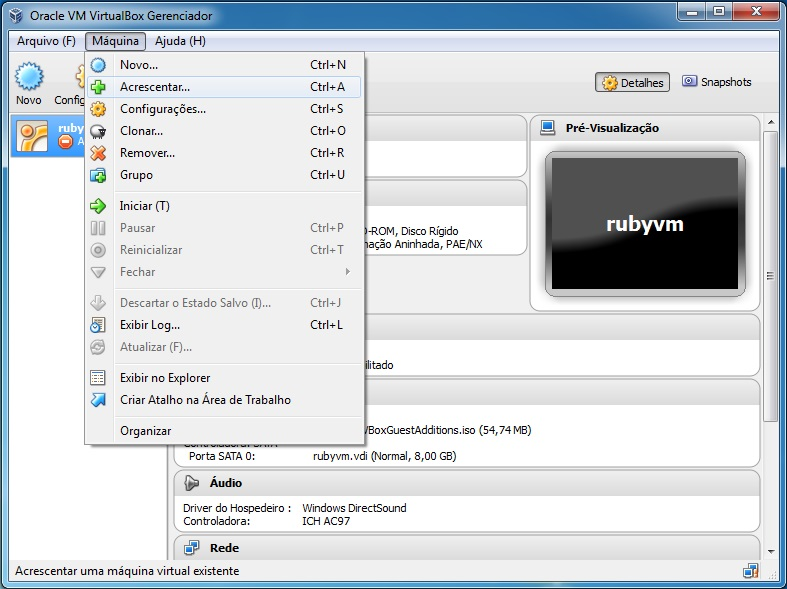
\includegraphics[width=0.45\textwidth]{devops/imagens/virtual-box-acrescentar-vm-1.jpg}
    \end{figure}
    
    \item Abra o arquivo da máquina virtual \verb!rubyvm.vdi! na pasta \verb|Downloads\rubyvm\rubyvm|.
    \begin{figure}[h!]
      \centering
      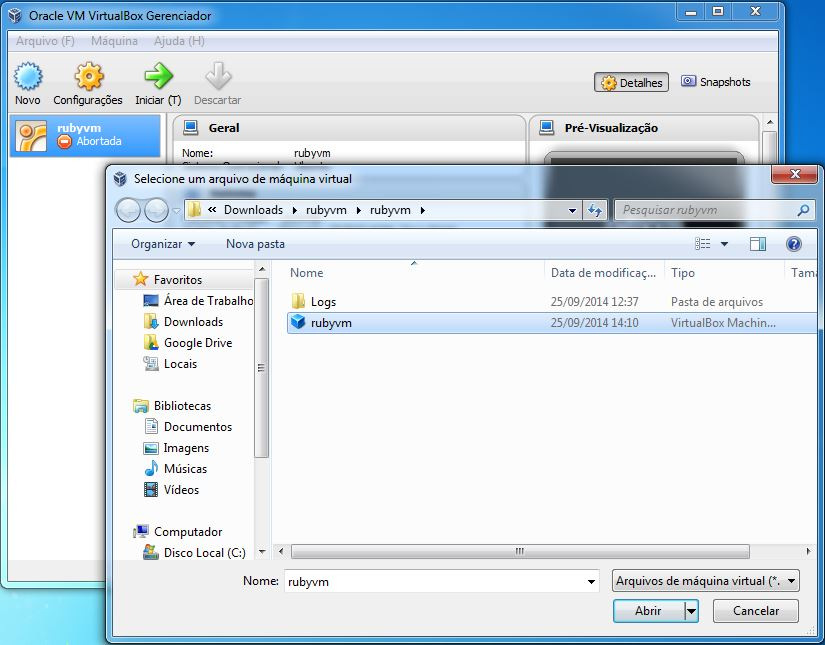
\includegraphics[width=0.45\textwidth]{devops/imagens/virtual-box-acrescentar-vm-2.jpg}
    \end{figure}

 \framebreak
    \item Selecione a máquina virtual \verb!rubyvm! e a inicie clicando no ícone \verb!Iniciar(T)!.
    \begin{figure}[h!]
      \centering
      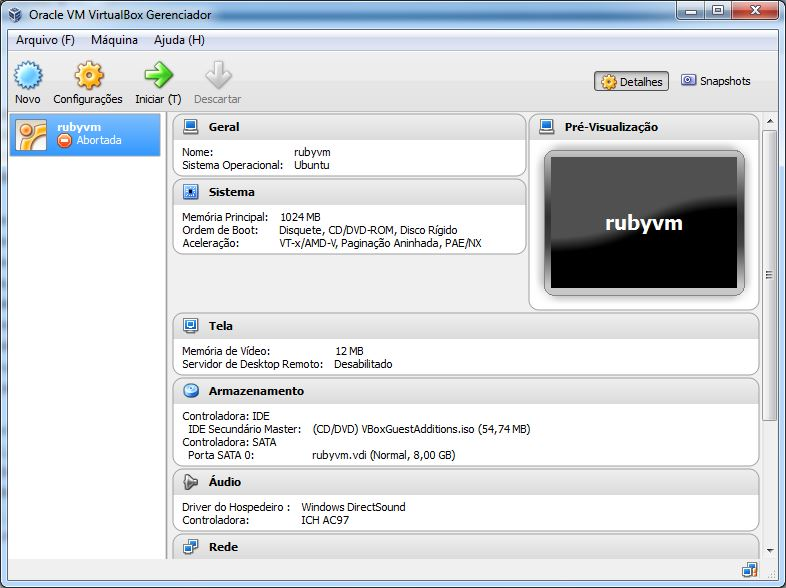
\includegraphics[width=0.45\textwidth]{devops/imagens/virtual-box-acrescentar-vm-3.jpg}
    \end{figure}
    
 \framebreak
    \item Após alguns segundos a tela de conexão do \verb!Ubuntu! será mostrada. O usuário e senha
      para se conectar à máquina virtual são respectivamente \alert{puc} e \alert{puc}.
    \begin{figure}[h!]
      \centering
      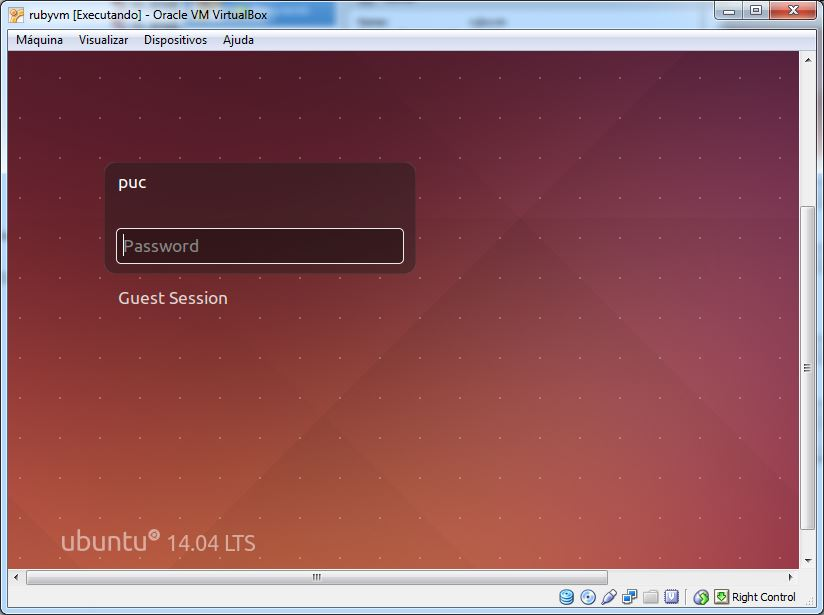
\includegraphics[width=0.45\textwidth]{devops/imagens/virtual-box-acrescentar-vm-4.jpg}
    \end{figure}
    
  \end{enumerate}
   
\end{frame}
